% Created 2017-02-06 Mon 10:39
% Intended LaTeX compiler: pdflatex
\documentclass[presentation]{beamer}
\usepackage[utf8]{inputenc}
\usepackage[T1]{fontenc}
\usepackage{graphicx}
\usepackage{grffile}
\usepackage{longtable}
\usepackage{wrapfig}
\usepackage{rotating}
\usepackage[normalem]{ulem}
\usepackage{amsmath}
\usepackage{textcomp}
\usepackage{amssymb}
\usepackage{capt-of}
\usepackage{hyperref}
\usetheme{AnnArbor}
\usecolortheme{}
\author{Zheng Tian}
\date{}
\title{Emacs, Org-Mode, and Reproducible Research}
\hypersetup{
 pdfauthor={Zheng Tian},
 pdftitle={Emacs, Org-Mode, and Reproducible Research},
 pdfkeywords={},
 pdfsubject={},
 pdfcreator={Emacs 25.1.1 (Org mode 9.0.3)},
 pdflang={English}}
\begin{document}

\maketitle
\begin{frame}{Outline}
\setcounter{tocdepth}{1}
\tableofcontents
\end{frame}



\section*{Introduction}
\label{sec:orgebbf723}


\section*{Emacs}
\label{sec:orgbf7100f}

\begin{frame}[label={sec:org586dce5}]{What is Emacs? A text editor.}
GNU Emacs is a free, portable, extensible text editor.

\begin{itemize}
\item Free: Open source, freely copyable and redistributable.
\item Portable: Run on many machines under different operating systems.
\item Extensible: Customizable for all aspect and  many contributed packages,
\end{itemize}
\end{frame}


\subsection*{Emacs is beyond a text editor}
\label{sec:orgd918eb2}

\begin{frame}[label={sec:orgb4fad2f}]{Emacs is IDE for programming languages}
\begin{itemize}
\item Edit code with syntax highlighting
\item Execute code within Emacs
\end{itemize}

\begin{figure}[htbp]
\centering
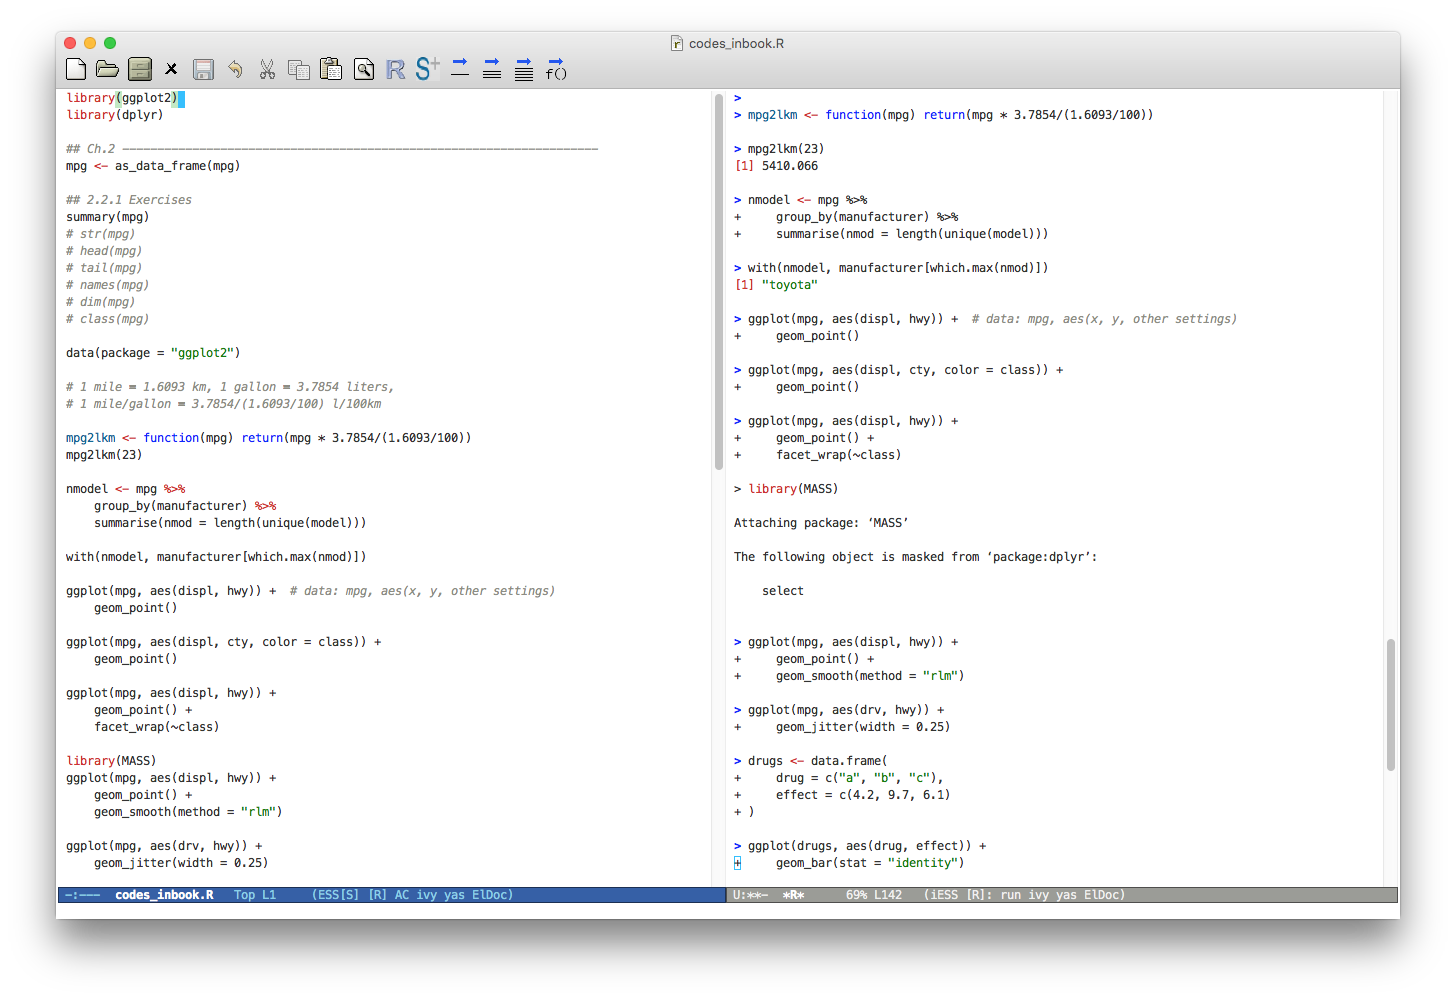
\includegraphics[width=0.8\textwidth]{figure/r_example.png}
\caption{An illustration of the ESS mode}
\end{figure}
\end{frame}

\begin{frame}[label={sec:org5dd4b0d}]{Emacs is an operating system}
\begin{itemize}
\item Emacs is an operating system, easily managing files and folders
within a dired-directory interface.
\end{itemize}

\begin{figure}[htbp]
\centering
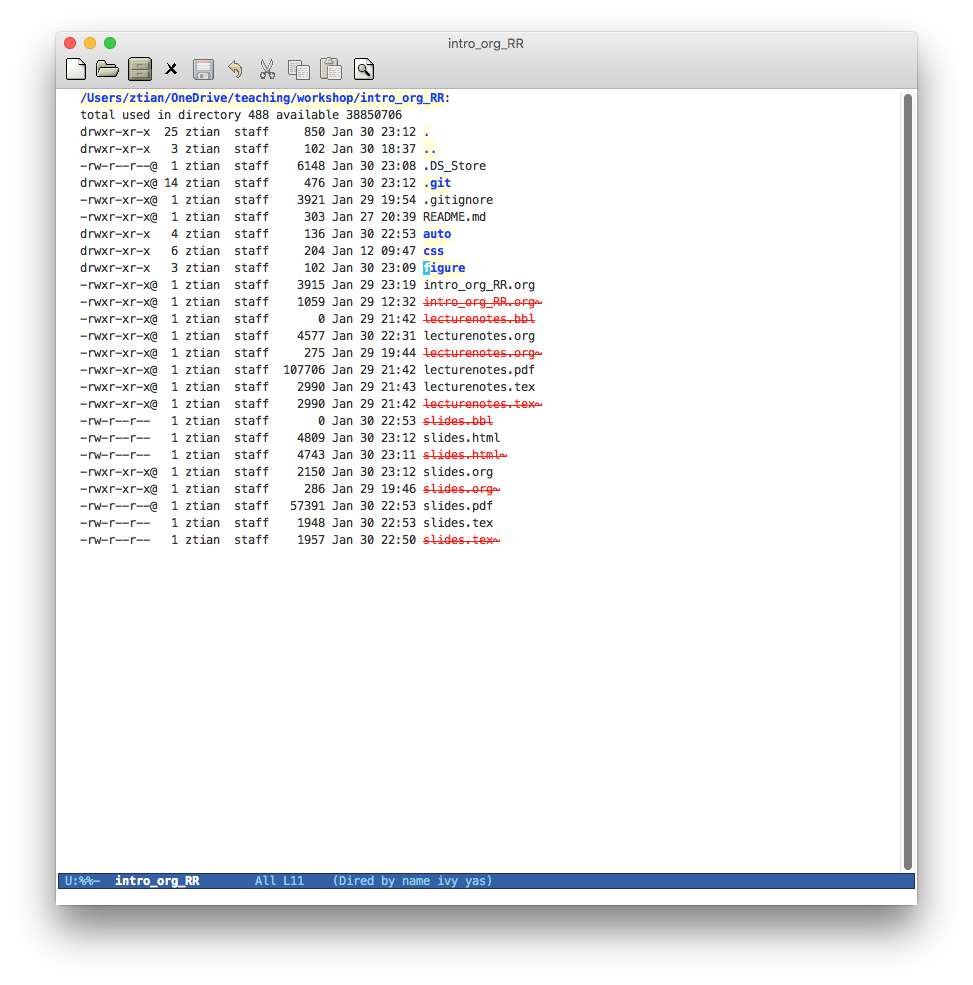
\includegraphics[width=0.8\textwidth]{figure/dired_example.png}
\caption{Emacs as an operating system with the dired mode}
\end{figure}
\end{frame}

\begin{frame}[label={sec:orge492643}]{Emacs can do many other things}
\begin{itemize}
\item Emacs can do spell checking, reading news, checking and sending
emails, etc., through plenty of contributed packages.
\item Most importantly, Emacs enable researchers to manage research
project, take notes, and write dynamic documentation.
\end{itemize}
\end{frame}


\subsection*{Installation and Configuration}
\label{sec:org9720bf9}

\begin{frame}[label={sec:orgabb7179}]{Installation}
\begin{itemize}
\item Homepage of GNU Emacs: \url{https://www.gnu.org/software/emacs/}

\item Vincent Goulet's binary files:
\url{http://vgoulet.act.ulaval.ca/en/emacs/}
\end{itemize}

\begin{NOTES}
I personally prefer the second option because it has already included
some of the mostly used packages.
\end{NOTES}
\end{frame}

\begin{frame}[fragile,label={sec:orgf384717}]{Configuration}
 Emacs is customizable and all customized configuration can be done
with either a \texttt{.emacs} file or \texttt{init.el} under the directory
\texttt{\textasciitilde{}/.emacs.d}.

With some settings, we can use an org file to organize and apply your
customization.
\end{frame}

\begin{frame}[fragile,label={sec:orgf4cd0f7}]{My settings}
 All my settings have been uploaded to Github from where you can
download or clone \texttt{git clone
https://github.com/zngtian/.emacs.d.git}.

\begin{block}{A peek of my settings}
\begin{description}
\item[{init.el}] \url{https://github.com/zngtian/.emacs.d/blob/master/init.el}
\item[{myconfig.org}] \url{https://github.com/zngtian/.emacs.d/blob/master/myconfig.org}
\end{description}
\end{block}
\end{frame}


\subsection*{Basic usage of Emacs}
\label{sec:orgdb65888}

\begin{frame}[label={sec:org30d29c9}]{Notation}
In Emacs documentation, we often see the following notations

\begin{description}
\item[{C-x}] Press Control key and x
\item[{M-x}] Press Alt key and x
\item[{RET}] Press the return key
\item[{SPC}] Press the space bar
\item[{ESC}] Press the escape key
\item[{S-<TAB>}] Press shift and tab keys
\end{description}
\end{frame}

\begin{frame}[label={sec:org59c486d}]{Buffer and windows}
The basic user interface of Emacs is in buffers and windows

\begin{figure}[htbp]
\centering
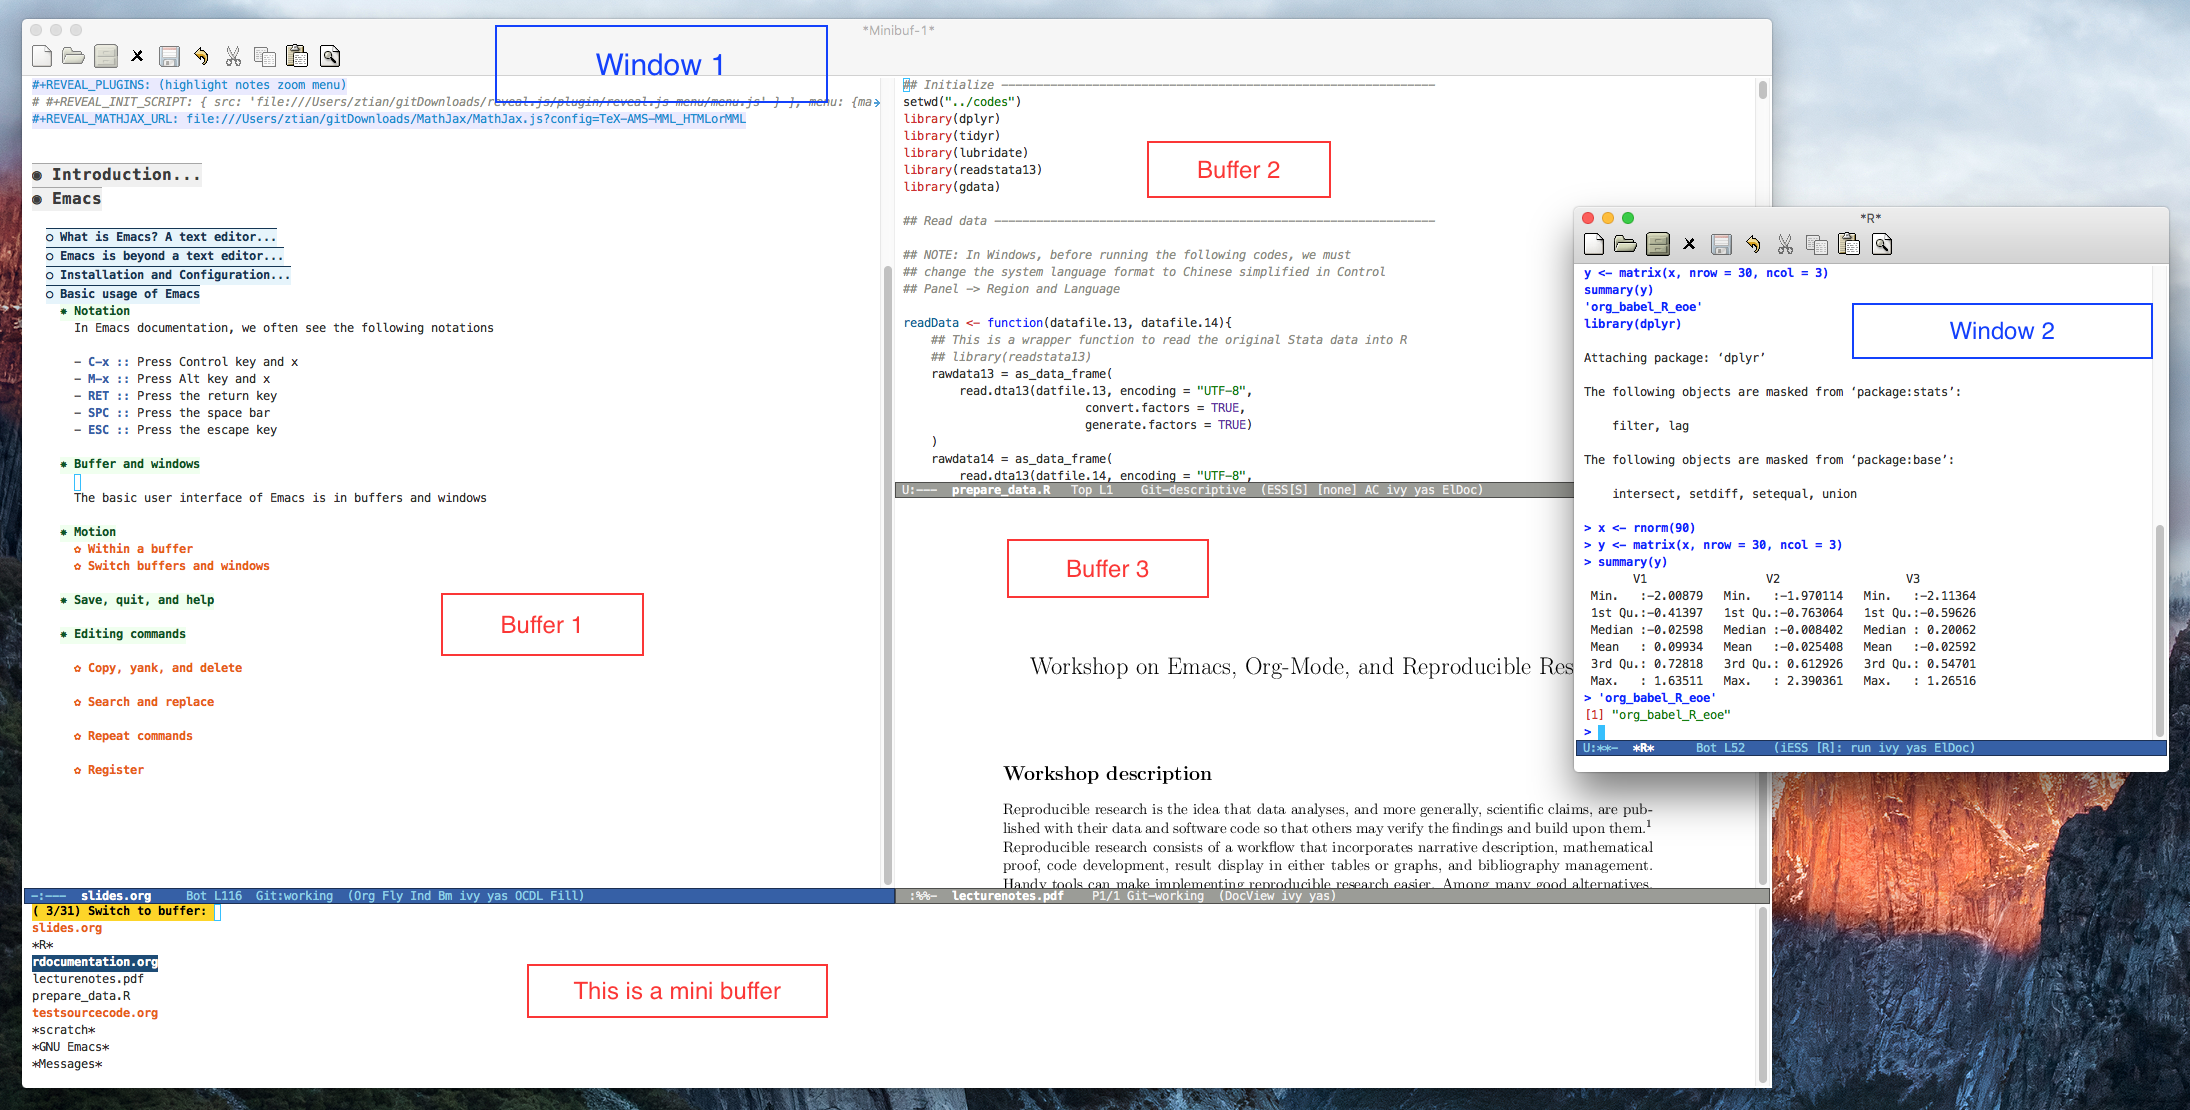
\includegraphics[width=1.0\textwidth,height=0.8\textheight]{figure/buffer_example.png}
\caption{An example of Emacs buffers and windows}
\end{figure}

\begin{NOTES}
Demonstrate some operations on Emacs in this section.
\end{NOTES}
\end{frame}

\begin{frame}[label={sec:org47e65a3}]{Motion within a buffer}
\begin{itemize}
\item C-f and M-f: move forward by one character and by one word
\item C-b and M-b: move backward by one letter and by one word
\item C-n and C-p: move downward and upward
\item C-v and M-v: scroll down and up
\item M-< and M->: move to the start and to the end of a buffer
\end{itemize}
\end{frame}

\begin{frame}[label={sec:org0802c6e}]{Switch buffers and windows}
\begin{itemize}
\item C-x 2: open a new buffer
\item C-x 0: close the current buffer
\item C-x b: switch to a buffer
\item C-x o: switch between two opened buffers
\item C-x 4 b: switch to a buffer and open it as a new one
\item C-x 5 2 and C-x 5-0: open and close a new window
\end{itemize}
\end{frame}

\begin{frame}[label={sec:orgdb0b688}]{Open, save, quit, and help}
\begin{itemize}
\item C-x C-f: open a new file
\item C-x C-s: save the current buffer
\item C-x s: save all files
\item C-g: cancel the currently invoked command. VERY IMPORTANT!
\item C-x C-c: exit Emacs
\item C-h ?/m/a: get help
\end{itemize}
\end{frame}

\begin{frame}[label={sec:orgdb2ccf0}]{Copy, yank, and delete}
\begin{itemize}
\item C-SPC: set a mark and move the cursor around to select a region
\item C-w: kill (cut)
\item M-w: copy
\item C-y: yank (paste)
\item DEL and C-d: delete a character backward and forward
\item M-DEL and M-d: delete a word backward and forward
\item C-k: kill a line.
\item C-x u: undo the previous editing.
\end{itemize}
\end{frame}

\begin{frame}[label={sec:org48f5bf3}]{Tutorial and cheat sheet}
\begin{itemize}
\item C-h t: open the complete tutorial

\item A guided tour: \url{https://www.gnu.org/software/emacs/tour/}

\item Cheat sheet: \url{https://www.gnu.org/software/emacs/refcards/pdf/refcard.pdf}
\end{itemize}
\end{frame}


\section*{Org-Mode}
\label{sec:orgdf3343a}

\begin{frame}[label={sec:org655b048}]{What is org-mode}
Org mode is one of the most popular contributed packages in Emacs. It
can accomplish a variety of work including, but not limited to,

\begin{itemize}
\item taking notes with structured documentation,
\item assigning tasks and scheduling them,
\item editing tables and doing calculation,
\item exporting to pdf, html, odt files,
\item \alert{working with source code}.
\end{itemize}
\end{frame}


\subsection*{Structured document}
\label{sec:orga05ef52}

\begin{frame}[fragile,label={sec:org2b70a3f}]{Headline}
 \begin{verbatim}
* Top level headline
** Second level
*** 3rd level
    some text
*** 3rd level
    more text

* Another top level headline
\end{verbatim}

\begin{itemize}
\item Hit <TAB> key at a headline to see and hide the content under it
\item S-<TAB>: global cycling.
\item M-left and M-right: promote and demote a heading
\item C-c C-p, C-c C-n, C-c C-f, and C-c C-b: move up and down between
headlines
\item Use org-bullets to make it prettier.
\end{itemize}
\end{frame}

\begin{frame}[fragile,label={sec:orgae52a35}]{Lists}
 \begin{verbatim}
- Unordered list
  + Item 1
  + Item 2
- Ordered list
  1. first thing
  2. second thing
  3. third thing
- Description
  - Tom :: a cat
  - Jerry :: a mouse
- List with check box
  - [X] Do this
  - [ ] Do that
\end{verbatim}
\end{frame}


\subsection*{Special elements}
\label{sec:org7923a3f}

\begin{frame}[fragile,label={sec:org58362df}]{Links}
 \begin{itemize}
\item The basic syntax for a link:
\begin{verbatim}
[[link][description]] or [[link]]
\end{verbatim}

\item Internal link: \hyperlink{sec:orgae52a35}{Lists}
\begin{verbatim}
[[Lists]]
\end{verbatim}

\item External link: \url{slides.tex}
\begin{verbatim}
[[file:slides.tex]]
\end{verbatim}

\item URL: \url{http://rri.wvu.edu/}
\begin{verbatim}
[[http://rri.wvu.edu/]]
\end{verbatim}
\end{itemize}
\end{frame}

\begin{frame}[fragile,label={sec:org3e9b803}]{Blocks}
 \begin{itemize}
\item Blocks are defined by \texttt{\#+BEGIN\_... and \#+END\_...}

\item The CENTER block

\begin{center}
This sentence will be centered in the exported file
\end{center}

\begin{verbatim}
#+BEGIN_CENTER
This sentence will be centered in the exported file
#+END_CENTER
\end{verbatim}

\item The QUOTE block

\begin{quote}
Everything should be made as simple as possible,
but not any simpler -- Albert Einstein
\end{quote}

\begin{verbatim}
#+BEGIN_QUOTE
 Everything should be made as simple as possible,
 but not any simpler -- Albert Einstein
 #+END_QUOTE
\end{verbatim}
\end{itemize}
\end{frame}

\begin{frame}[fragile,label={sec:org23aaed1}]{Mathematics}
 Org mode can contain \LaTeX{} math fragments that don't need any special
marking. Just do as in \LaTeX{}.

\begin{verbatim}
\begin{equation}
    x=\sqrt{b}
\end{equation}

If $a^2=b$ and \( b=2 \), then the solution must be
either $$ a=+\sqrt{2} \text{ or }  a=-\sqrt{2} $$
\end{verbatim}

\begin{equation}
    x=\sqrt{b}
\end{equation}

If \(a^2=b\) and \(b=2\), then the solution must be
either $$ a=+\sqrt{2} \text{ or }  a=-\sqrt{2} $$
\end{frame}

\begin{frame}[fragile,label={sec:orgbbff7c1}]{Table}
 \begin{itemize}
\item ‘|’ as the first non-whitespace character starts a table. The
following texts yield a table in HTML export

\begin{verbatim}
| Name  | Age | Score |
|-------+-----+-------|
| Peter |  17 |  1234 |
| Anna  |  25 |  4321 |
\end{verbatim}

\begin{center}
\begin{tabular}{lrr}
Name & Age & Score\\
\hline
Peter & 17 & 1234\\
Anna & 25 & 4321\\
\end{tabular}
\end{center}
\end{itemize}
\end{frame}

\begin{frame}[fragile,label={sec:org278ced3}]{Calculation in a table}
 \begin{itemize}
\item We can define formula for a field, a row, or a column by starting a
field with "="
\end{itemize}

\begin{verbatim}
| Name  | Age | Score |
|-------+-----+-------|
| Peter |  17 |  1234 |
| Anna  |  25 |  4321 |
|       |  21 |  5555 |
#+TBLFM: @4$2=vmean(@2..@3)::@4$3=vsum(@2..@3)
\end{verbatim}

\begin{center}
\begin{tabular}{lrr}
Name & Age & Score\\
\hline
Peter & 17 & 1234\\
Anna & 25 & 4321\\
 & 21 & 5555\\
\end{tabular}
\end{center}
\end{frame}


\begin{frame}[fragile,label={sec:orgba15100}]{Exporting}
 \begin{itemize}
\item An org file can be exported to a variety of formats, including
latex, beamer, html, odt, etc.
\item \texttt{C-c C-e}: start the export dispatcher.
\item Then you can select from several options. Try \texttt{C-c C-e l O} to
generate the beamer file.
\item This presentation is exported with the \texttt{og-reveal} package.
\item Export settings can be set using some keywords, such as
\texttt{\#+TITLE, \#+AUTHOR, \#+OPTIONS, \#+LATEX\_HEADER, \#+HTML\_HEADER},
etc.
\end{itemize}
\end{frame}


\subsection*{Tasks and agenda view}
\label{sec:org3d0c44c}

\begin{frame}[label={sec:org05568ed}]{A sneak peek of my agenda}
Org mode is not just a text editor that can include a rich variety of
elements but also a handy tool to plan daily life and manage
research projects.

\begin{figure}[htbp]
\centering
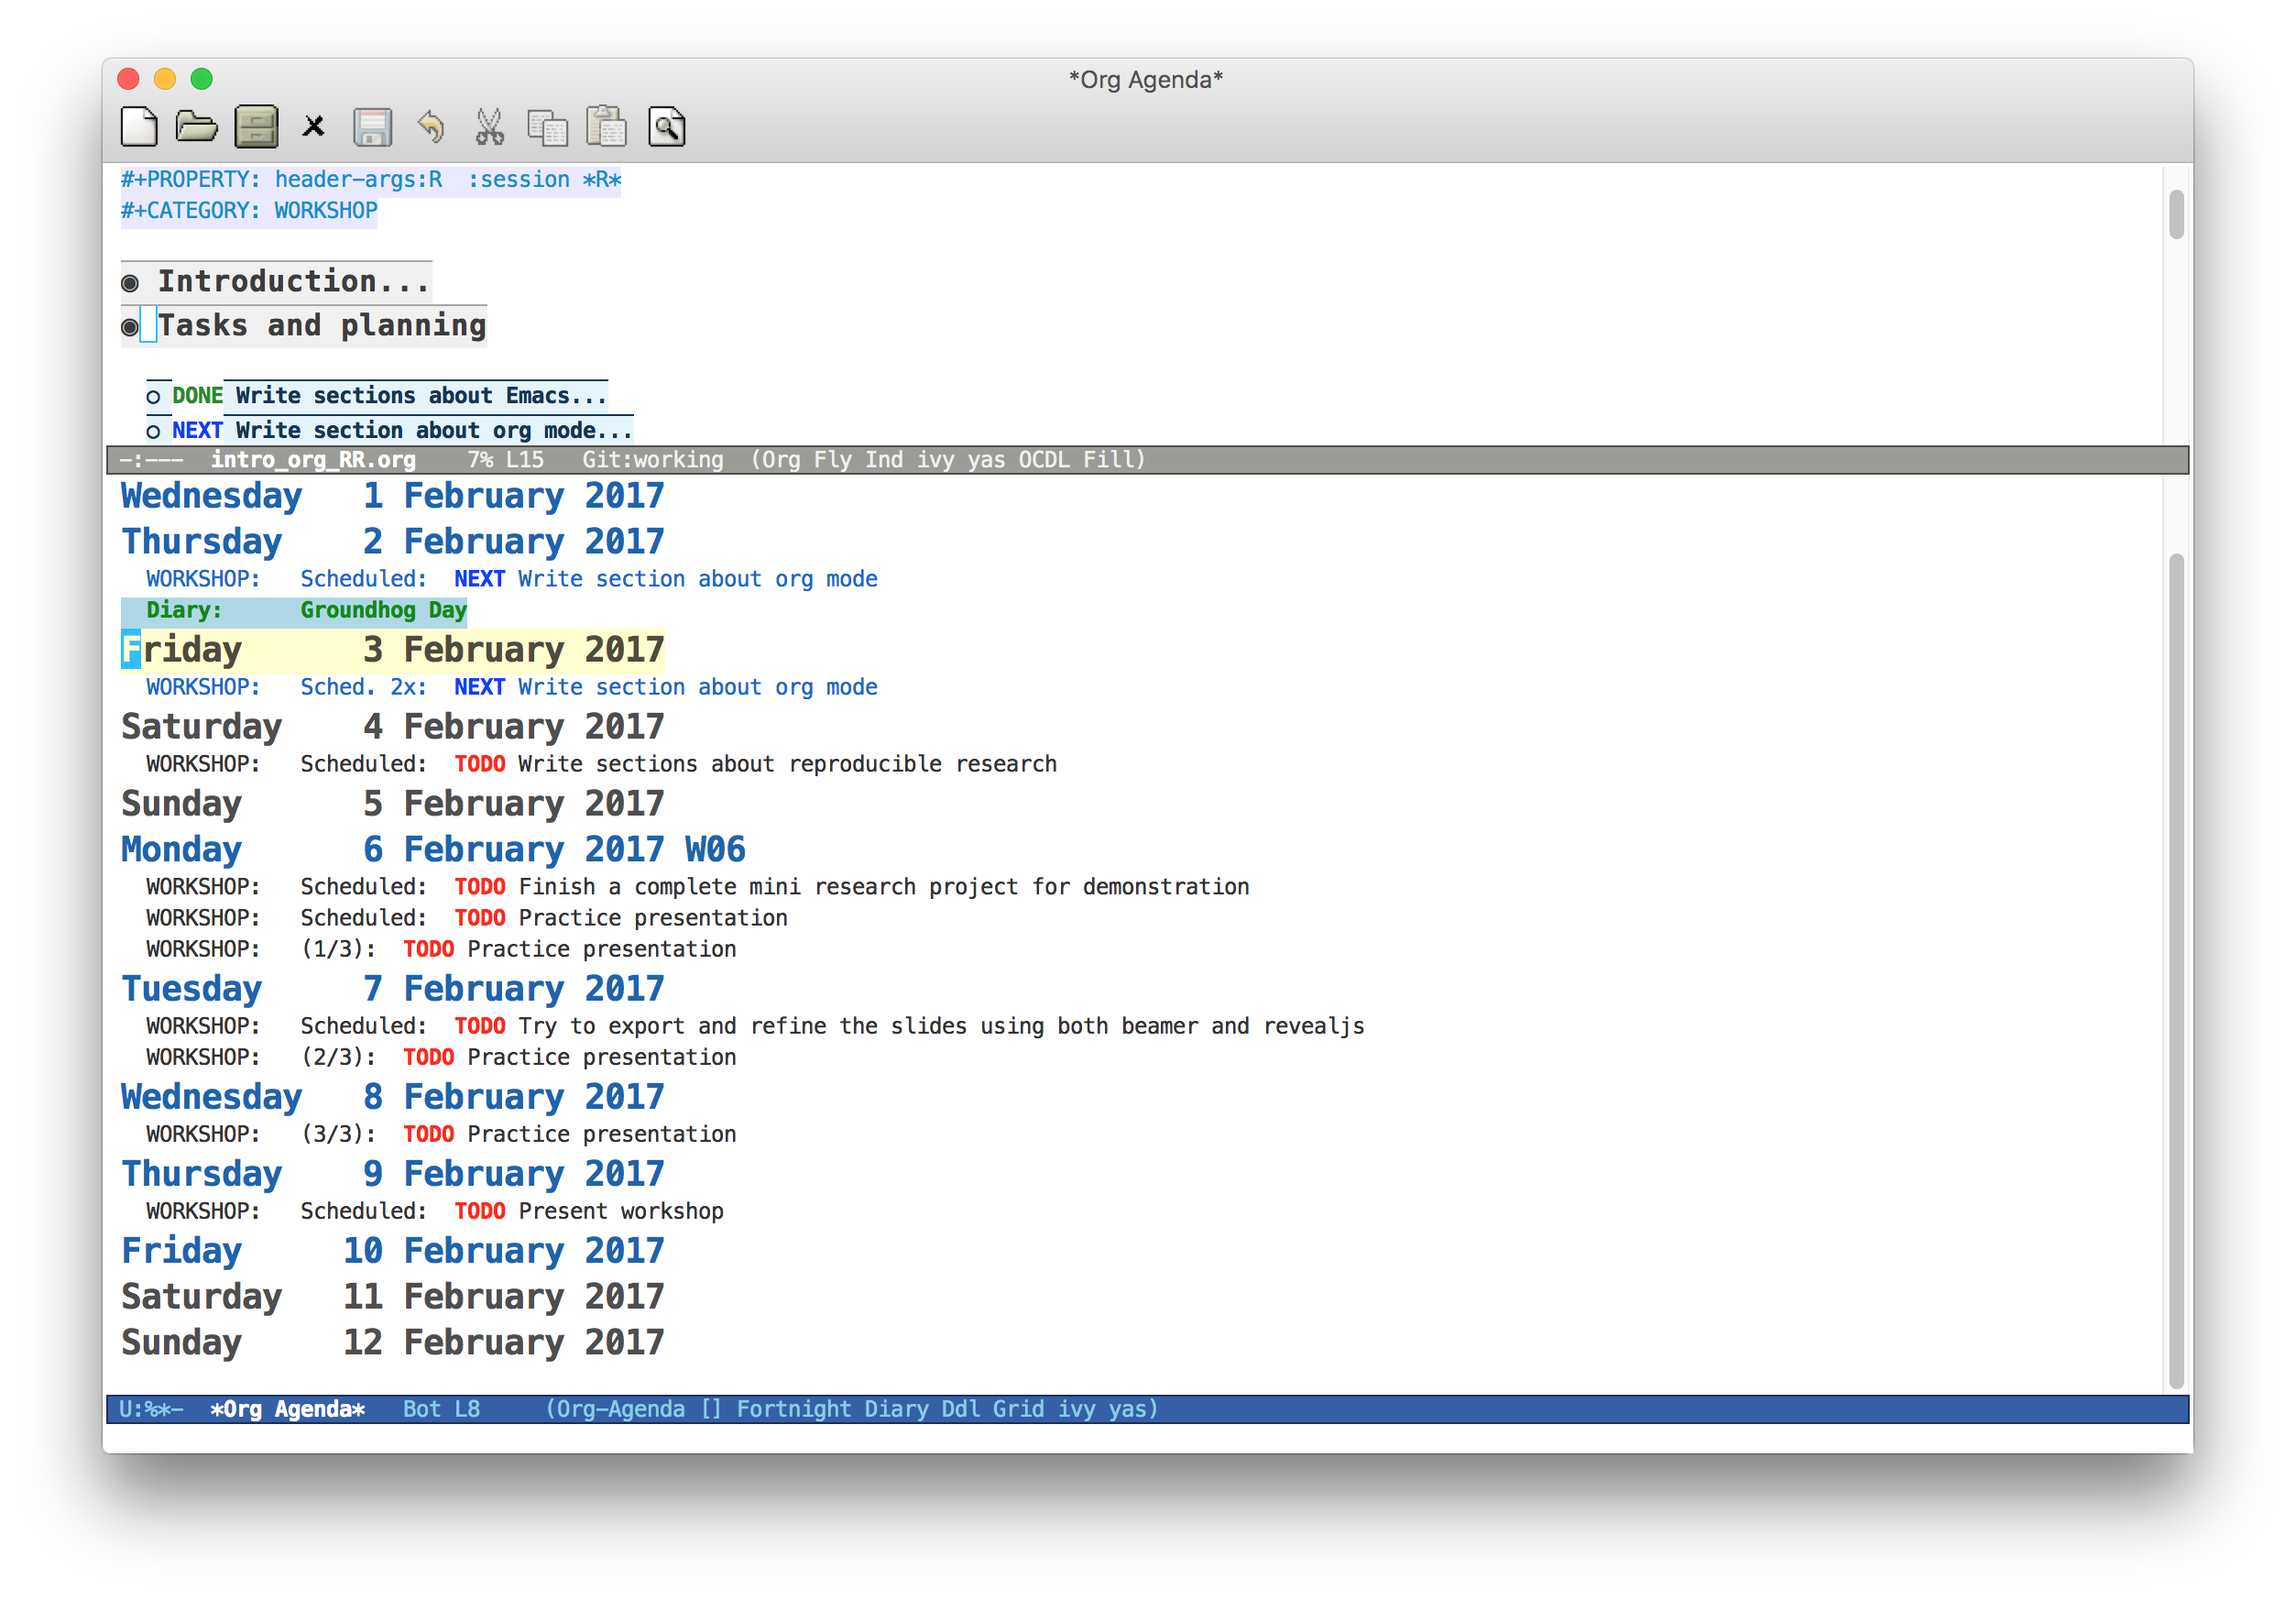
\includegraphics[width=0.6\textwidth,height=0.5\textheight]{figure/agenda_example.png}
\caption{An illustration of agenda view}
\end{figure}
\end{frame}


\begin{frame}[fragile,label={sec:org2188ae0}]{To-do items}
 TODO items in org mode are headlines defined by TODO keywords after
asterisks.

\begin{verbatim}
* [#A] TODO Do this first.
* DONE This task has been done
\end{verbatim}

\begin{itemize}
\item M-S RET: quick enter a TODO item
\item S-right/left: cycle through TODO status
\item S-up/down: cycle through priorities.
\end{itemize}
\end{frame}


\begin{frame}[fragile,label={sec:org0427206}]{Schedule and deadline}
 We can set schedule and deadline to TODO items.

\begin{itemize}
\item C-c C-s: set a day and time to begin doing this item
\item C-c C-d: set a deadline
\item Time stamps are generated using the calendar minor mode.
\end{itemize}

\begin{verbatim}
* [#A] TODO Do this first.
  SCHEDULED: <2017-02-03 Fri>

* DONE This task has been done
  DEADLINE: <2017-02-03 Fri>
\end{verbatim}
\end{frame}


\begin{frame}[label={sec:org3d88727}]{Agenda view}
All TODO items, schedules, and deadlines can be viewed in the Agenda
view in org mode.

\begin{itemize}
\item C-c a a: start the agenda view
\item C-c a t: see all TODO items
\item C-c a m: filter TODO items by tags
\end{itemize}

Within the agenda view, you can filter by tag, change the status, and
go to the headline of a TODO item.
\end{frame}


\section*{Reproducible research with org-mode}
\label{sec:org1ab3179}

\subsection*{Reproducible research: basics}
\label{sec:orgf973b40}

\begin{frame}[label={sec:org532b405}]{What is reproducible research?}
\begin{quote}
The data and code used to make a finding are available and they are
sufficient for an independent researcher to recreate the finding.
-- Gandrud (2015)
\end{quote}
\end{frame}


\begin{frame}[label={sec:org663c9aa}]{Why should we do reproducible research?}
\begin{block}{For readers}
\begin{itemize}
\item Easy for reviewers to test and validate your findings.
\item Easy for readers to reuse your code in their research.
\item Make your paper a reliable citation.
\end{itemize}
\end{block}

\begin{block}{For ourselves}
\begin{itemize}
\item Easy for us to tract and retrospect what we have done.
\item Helpful to have good research habits and workflow.
\item Facilitating team work.
\end{itemize}
\end{block}
\end{frame}


\begin{frame}[label={sec:org873bd09}]{What is a workflow of reproducible research?}
\begin{figure}[htbp]
\centering
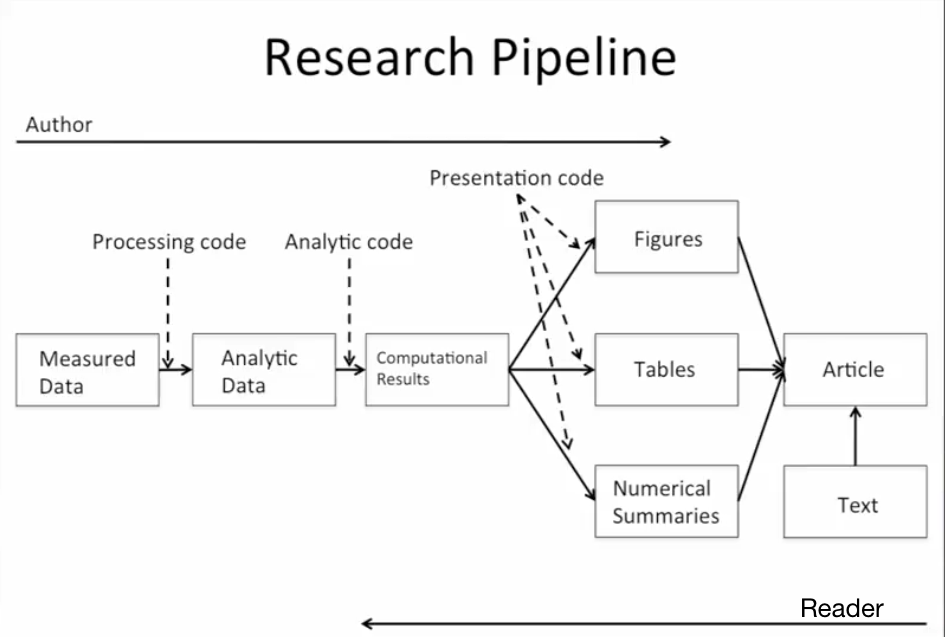
\includegraphics[width=0.8\textwidth,height=0.7\textheight]{figure/research_pipline.png}
\caption{A workflow of reproducible research (Source: Peng (2015))}
\end{figure}
\end{frame}


\begin{frame}[label={sec:org6032e56}]{What are necessary elements of reproducible research?}
Roger Peng (2015) summarizes four essential elements to make results
reproducible:
\begin{itemize}
\item Analytical data
\item Analytical code
\item Documentation
\item Distribution
\end{itemize}
\end{frame}


\subsection*{Literate programming}
\label{sec:org3c10dbd}

\begin{frame}[label={sec:org3b9f54c}]{What is literate programming?}
Literate programming (Donald Knuth, 1992) is the central part of
reproducible research.


Typically, literate programming involves the following three steps
(Xie, 2015):
\begin{enumerate}
\item parse the source document and separate the code from narratives;
\item execute the source code and return results;
\item mix results from the source code with the original narratives.
\end{enumerate}
\end{frame}

\begin{frame}[fragile,label={sec:orga9239e6}]{Available tools for literate programming}
 \begin{itemize}
\item WEB (Knuth, 1983)
\item Noweb (Ramsey, 1994)
\item \texttt{roxygen2} (Wickham et al., 2015)
\item \texttt{knitr} (Xie, 2015b)
\item Jupyter(IPython) Notebook
\item Emacs org mode
\end{itemize}
\end{frame}


\subsection*{Literate programming in with Org-mode}
\label{sec:orgd40efab}

\begin{frame}[fragile,label={sec:orgb6904d5}]{Source code block}
 The basic structure of code blocks is as follows

\begin{verbatim}
#+NAME: <name>
#+BEGIN_SRC <language> <switches> <header arguments>
   <body>
#+END_SRC
\end{verbatim}

The structure of an inline code block is

\begin{verbatim}
src_<language>[<header arguments>]{<body>}
\end{verbatim}
\end{frame}

\begin{frame}[fragile,label={sec:org807e1c8}]{Basic settings}
 \begin{verbatim}
#+BEGIN_SRC emacs-lisp :eval no
  (org-babel-do-load-languages
   'org-babel-load-languages
     '((R . t)
       (python . t)
       (emacs-lisp . t)
       (calc . t)
       (latex . t)
       (org . t)
       (sh . t)))

    (setq org-confirm-babel-evaluate nil)
#+END_SRC
\end{verbatim}
\end{frame}

\begin{frame}[label={sec:org634bbee}]{Header arguments}
Header arguments fine-tune the behaviors of a source block.

\begin{center}
\begin{tabular}{ll}
Header arguments & Example\\
\hline
:exports & :exports results or :exports none\\
:results & :results value table or :results silent\\
:eval & :eval no\\
:cache & :cache yes\\
:file & :file ./img/figure1.png\\
\end{tabular}
\end{center}
\end{frame}

\begin{frame}[fragile,label={sec:org08abd38}]{Results in raw format}
 \begin{verbatim}
#+BEGIN_SRC R :exports both :results output
library(ggplot2)
head(mpg[1:5])
#+END_SRC

#+RESULTS:
:   manufacturer model displ year cyl
: 1         audi    a4   1.8 1999   4
: 2         audi    a4   1.8 1999   4
: 3         audi    a4   2.0 2008   4
: 4         audi    a4   2.0 2008   4
: 5         audi    a4   2.8 1999   6
: 6         audi    a4   2.8 1999   6
\end{verbatim}
\end{frame}


\begin{frame}[fragile,label={sec:org738bc10}]{Results in org tables}
 \begin{verbatim}
#+BEGIN_SRC R :exports results :results value table :colnames yes :cache yes
head(mpg[1:5])
#+END_SRC

#+RESULTS[f45a5d1174dd12cdb343701a0868203eda23a5bc]:
| manufacturer | model | displ | year | cyl |
|--------------+-------+-------+------+-----|
| audi         | a4    |   1.8 | 1999 |   4 |
| audi         | a4    |   1.8 | 1999 |   4 |
| audi         | a4    |     2 | 2008 |   4 |
| audi         | a4    |     2 | 2008 |   4 |
| audi         | a4    |   2.8 | 1999 |   6 |
| audi         | a4    |   2.8 | 1999 |   6 |
\end{verbatim}
\end{frame}

\begin{frame}[fragile,label={sec:org045ad4f}]{Results in figures}
 \begin{verbatim}
#+BEGIN_SRC R :exports both :results output graphics :file mpg.png
  ggplot(mpg, aes(displ, cty, colour = class)) +
      geom_point()
#+END_SRC

#+ATTR_HTML: :width 600 :height 500
#+ATTR_LATEX: :width 0.6\textwidth :height 0.6\textheight
#+RESULTS:
[[file:mpg.png]]
\end{verbatim}
\end{frame}

\begin{frame}[label={sec:org3f8e3d6}]{The figure generated}
\begin{figure}[htbp]
\centering
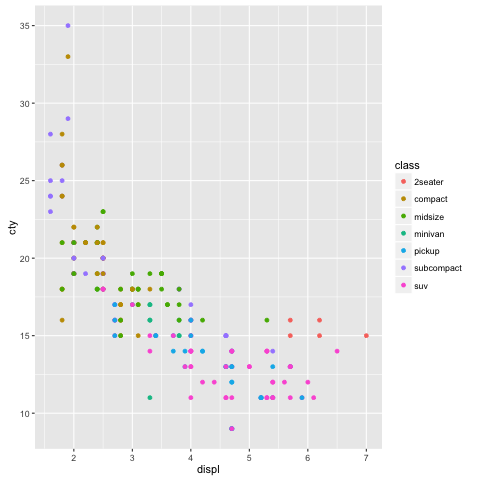
\includegraphics[width=0.5\textwidth,height=0.5\textheight]{mpg.png}
\caption{The Scatterplot Between the Engine Displacement and City MPG}
\end{figure}
\end{frame}

\begin{frame}[fragile,label={sec:org224e38b}]{Results in latex}
 \begin{verbatim}
#+BEGIN_SRC R :exports both :results output latex
library(stargazer)
stargazer(mpg, header = FALSE)
#+END_SRC

#+RESULTS:
#+BEGIN_EXPORT latex

% Table created by stargazer v.5.2 by Marek Hlavac, Harvard University. E-mail: hlavac at fas.harvard.edu
% Date and time: Mon, Feb 06, 2017 - 09:45:31
\begin{table}[!htbp] \centering
  \caption{}
  \label{}
\begin{tabular}{@{\extracolsep{5pt}}lccccc}
\\[-1.8ex]\hline
\hline \\[-1.8ex]
Statistic & \multicolumn{1}{c}{N} & \multicolumn{1}{c}{Mean} & \multicolumn{1}{c}{St. Dev.} & \multicolumn{1}{c}{Min} & \multicolumn{1}{c}{Max} \\
\hline \\[-1.8ex]
displ & 234 & 3.472 & 1.292 & 1.600 & 7.000 \\
year & 234 & 2,003.500 & 4.510 & 1,999 & 2,008 \\
cyl & 234 & 5.889 & 1.612 & 4 & 8 \\
cty & 234 & 16.859 & 4.256 & 9 & 35 \\
hwy & 234 & 23.440 & 5.955 & 12 & 44 \\
\hline \\[-1.8ex]
\end{tabular}
\end{table}
#+END_EXPORT
\end{verbatim}
\end{frame}

\begin{frame}[label={sec:org147990d}]{The \LaTeX{} table generated}

% Table created by stargazer v.5.2 by Marek Hlavac, Harvard University. E-mail: hlavac at fas.harvard.edu
% Date and time: Mon, Feb 06, 2017 - 09:45:31
\begin{table}[!htbp] \centering
  \caption{Summary Statistics of the =mpg= dataset}
  \label{}
\begin{tabular}{@{\extracolsep{5pt}}lccccc}
\\[-1.8ex]\hline
\hline \\[-1.8ex]
Statistic & \multicolumn{1}{c}{N} & \multicolumn{1}{c}{Mean} & \multicolumn{1}{c}{St. Dev.} & \multicolumn{1}{c}{Min} & \multicolumn{1}{c}{Max} \\
\hline \\[-1.8ex]
displ & 234 & 3.472 & 1.292 & 1.600 & 7.000 \\
year & 234 & 2,003.500 & 4.510 & 1,999 & 2,008 \\
cyl & 234 & 5.889 & 1.612 & 4 & 8 \\
cty & 234 & 16.859 & 4.256 & 9 & 35 \\
hwy & 234 & 23.440 & 5.955 & 12 & 44 \\
\hline \\[-1.8ex]
\end{tabular}
\end{table}
\end{frame}

\begin{frame}[label={sec:org7589f7f}]{An mini example of literate programming}
The following file is an example of reproducible research, which I
used in teaching Econometrics.

\url{example/replicate\_ch7.org}
\end{frame}

\begin{frame}[label={sec:org9e25517}]{Other useful packages}
\end{frame}

\begin{frame}[label={sec:org309270e}]{Windows users}
\end{frame}



\section*{Other useful modes in Emacs and org mode}
\label{sec:org8cb67c4}
\subsection*{ESS}
\label{sec:orgeb6f257}
\subsection*{AucTex}
\label{sec:orgf53a73f}
\subsection*{Magit}
\label{sec:org9c4bb02}
\subsection*{Org-ref}
\label{sec:org57881a5}

\section*{Reference}
\label{sec:orgfeaaf74}
\end{document}